\chapter{Approach}
\label{chp:apr}
This chapter explains the general structure and functionality of a system that is supposed to measure the received signal strength of every link in a network.
\TODO Write about what this chapter explains

\section{General Structure}
\label{chp:apr_general}

To measure the RSSI of each link all the nodes need to send messages. Since two nodes sending a message at the same time will distort the RSSI measurements we need to make sure that only one node sends a message at a given point in time. One approach to achieve this is the timeslot based method explained in Chapter 2.3. This method however includes an error inside its timeslots, resulting in a small delay between messages.
To eliminate the delay timeslots bring along a different approach is suggested in this thesis which is based on predefined predecessors for each node. Based on this a node will be able to send a message directly after receiving a message from its predecessor and at the same time making sure that only one node sends at a given point in time.\todo{Complex stuff because of not every node hearing the others}

The system consists of a base station with high processing power and a large memory as well as multiple distributed low power nodes. One of the nodes is the sink which is directly connected to the base station. The nodes are able to communicate with each other via radio, however not every node can hear all the other nodes. This structure is represented by Figure \ref{fig:architecture}. The fact that not every node is able to hear all the other nodes makes it a challenge to collect data from the network and to create a fitting schedule that defines predecessors for all the nodes inside the network. To be able to do so a first calibration phase is needed to create paths from every node to the sink and collect information about the connections between nodes. Then the information about the connections need to be collected at the sink and sent to the base station in a collection phase. When the base station received all the information it can create the schedule. After that the base station has to send the schedule to the sink that starts spreading it inside the network. 

Is the schedule spread and all the nodes know when to send their messages, the sampling of the RSSI can start. Therefore messages are sent according to the predecessors defined in the schedule. All the nodes receiving the messages are now able to measure the received signal strength to the sending node and store this information. When the schedule is completed another collection of the data is needed to gather the measured RSSI at the base station for further processing. When the collection is done, the system can start sampling again and then again collect the data until the system is stopped. This process is shown in Figure \ref{fig:processes}.    

\begin{figure}[htbp]
	\centering
	\begin{subfigure}[t]{0.4\textwidth}
		\centering
    		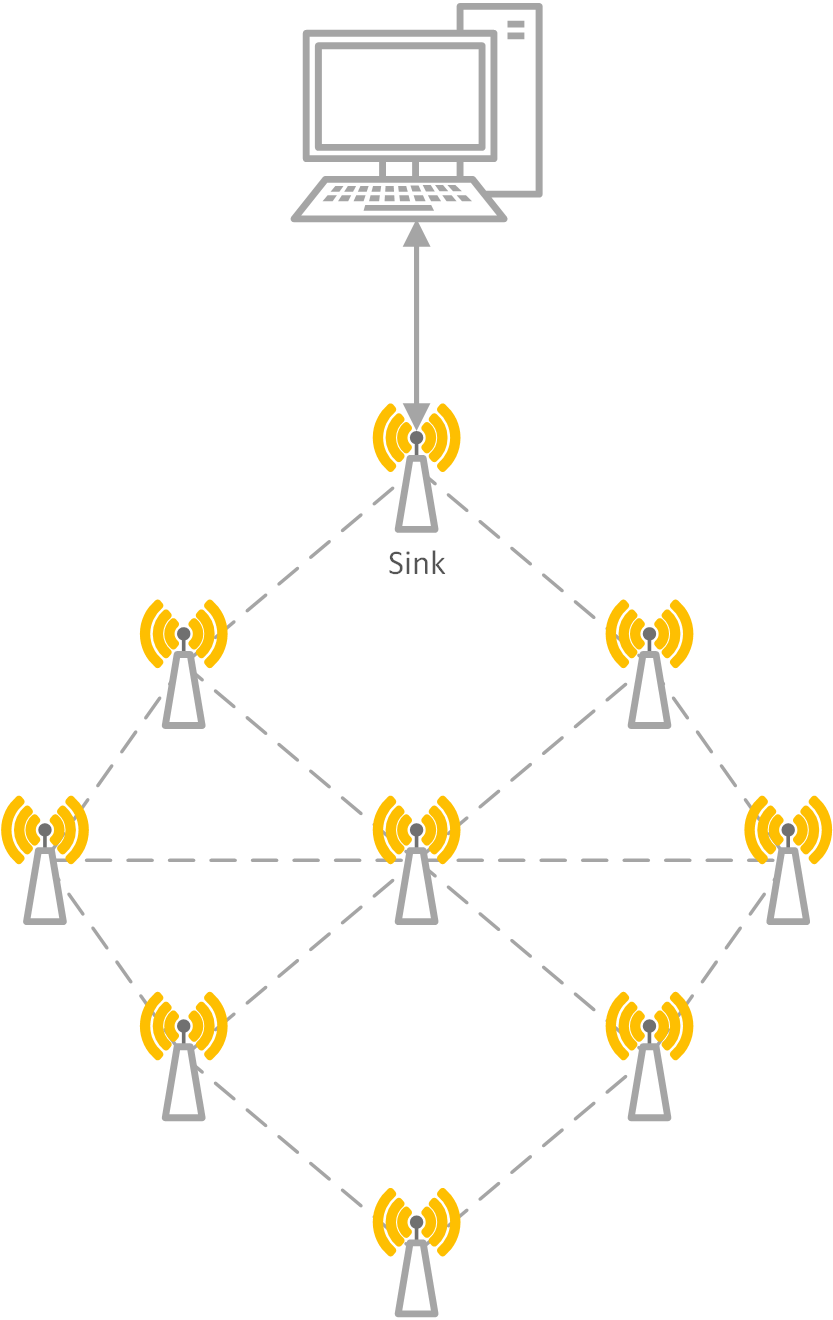
\includegraphics[scale=0.6]{content/images/Architecture}
   	 	\caption{The physical architecture of the system}
    	\label{fig:architecture}
    \end{subfigure}
    \quad
    \quad
    \quad
    \begin{subfigure}[t]{0.4\textwidth}
		\centering         
        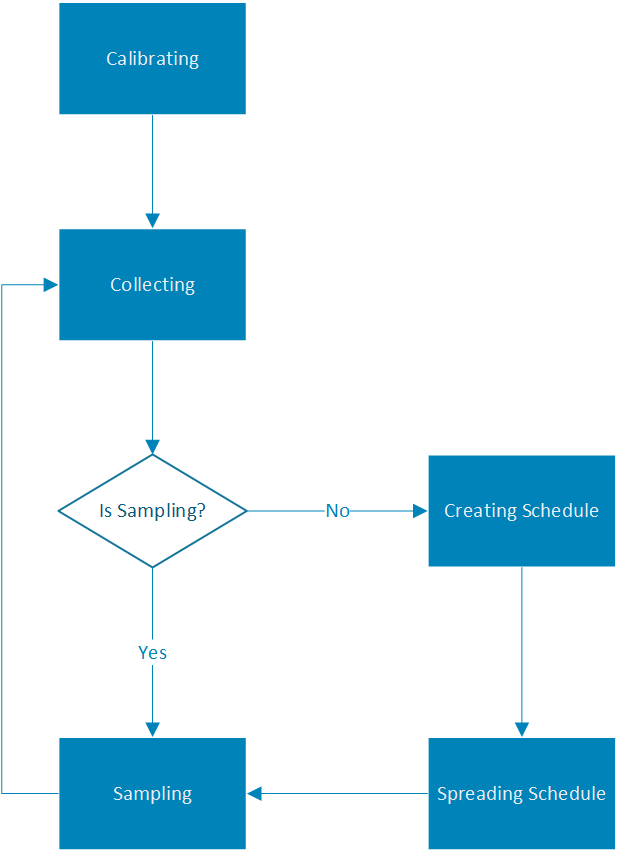
\includegraphics[scale=0.7]{content/images/GeneralAproachM}
        \caption{The general processes and the order in which they are executed}
        \label{fig:processes}
    \end{subfigure}
    \caption{}
\end{figure}

\section{Base Station}
\label{chp:apr_baseStation}
Since creating the schedule and storing and processing the data need a lot of processing power and storage, a base station is needed that fulfils these requirements. This base station needs to be connected to the sink so it can receive the collected data to process it. It also needs to be able to send data to the sink, so the schedule can be spread inside the network. \todo{kill this section?}
  
\section{Calibration}
\label{chp:apr_calibration}
The calibration has two tasks. It needs to figure out for each node individually which nodes a node has in its range and it needs to create paths to the sink. These paths will then later be used to send data to the sink or spread information inside the network. To achieve these tasks each node will send multiple messages without any specific pattern. \todo{define no pattern}

Each node needs to be able to keep track of the nodes in range. Therefore each node needs to have its own neighbour table. When a node receives a message it can put the node it received the message from inside that neighbour table. All the neighbour tables will later be the basis to create the schedule.

To later collect data from each individual node at the sink, each node needs to know to which node it needs to send its data to so it will reach the sink. This node is the parent of the node. Moreover to spread data inside the network each node also needs to know which nodes will send to itself in direction of the sink. These nodes are the children of a node. When each node found its parent and its children all the paths together will form a tree structure with the sink as the root.

To find the parents for the nodes each node needs to save one extra information and also include this information inside the messages it sends. This information is the quality of the current path a node has to the sink. At the beginning all the nodes except the sink will initialize their path quality with the worst possible value. The sink will initialize its path quality with the best possible value. Now when a node receives a message it will add to the received path quality of the sending node the quality of the link between itself and the sending node to calculate the path quality to the sink for the node, if it would choose the sending node as its parent. The quality of a link is represented by the received signal strength. When the new path quality is calculated the node compares the calculated value with its current path quality. If the calculated value is better the node will set its parent to the sending node and save the new path quality. 

Now, to not only know the direction to the sink but also the direction going away from the sink the nodes need to find their children. Therefore each node will simply include their own parent inside the message it will send. A receiving node will now check if it is the parent of the sending node. If that is the case the receiving node can save the sending node as a child.       

\section{Collection}
\label{chp:apr_collection}

\begin{figure}[htbp]
	\label{fig:coll}
	\centering
	\begin{subfigure}[t]{0.4\textwidth}
		\centering
    		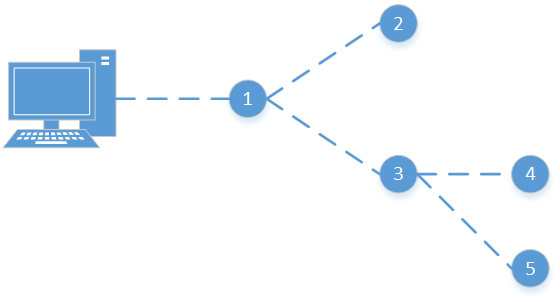
\includegraphics[scale=0.6]{content/images/Collection/Part0}
   	 	\caption{At the beginning all the nodes are unmarked and still have data to send}
    	\label{fig:coll0}
    \end{subfigure}
    \quad
    \quad	
	\begin{subfigure}[t]{0.4\textwidth}
		\centering
    		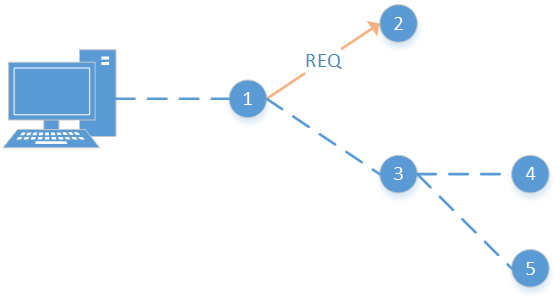
\includegraphics[scale=0.6]{content/images/Collection/Part1}
   	 	\caption{Node 1 sends the first request to node 2}
    	\label{fig:coll1}
    \end{subfigure}
    \quad
    \quad
    \begin{subfigure}[t]{0.4\textwidth}
		\centering         
        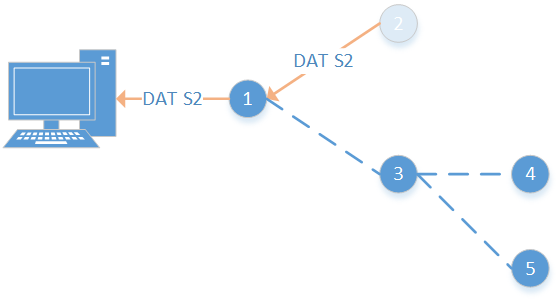
\includegraphics[scale=0.6]{content/images/Collection/Part2}
        \caption{Node 2 does not have any children so it sends its data and gets marked}
        \label{fig:coll2}
    \end{subfigure}
    \quad
    \quad
    \begin{subfigure}[t]{0.4\textwidth}
		\centering         
        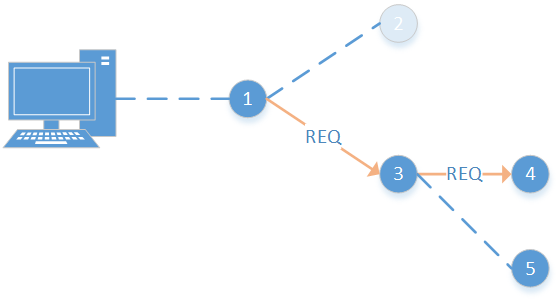
\includegraphics[scale=0.6]{content/images/Collection/Part3}
        \caption{Now node 2 is marked so node 1 sends a request to node 3, which forwards it to node 4}
        \label{fig:coll3}
    \end{subfigure}
    \quad
    \quad
    \begin{subfigure}[t]{0.4\textwidth}
		\centering         
        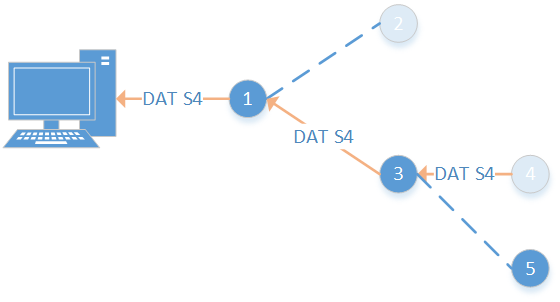
\includegraphics[scale=0.6]{content/images/Collection/Part4}
        \caption{Node 4 does not have any children so it sends its data and gets marked}
        \label{fig:coll4}
    \end{subfigure}
    \quad
    \quad
    \begin{subfigure}[t]{0.4\textwidth}
		\centering         
        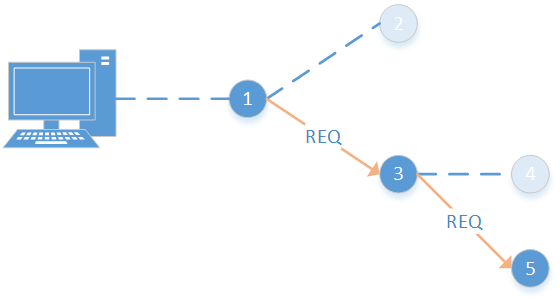
\includegraphics[scale=0.6]{content/images/Collection/Part5}
        \caption{Node 3 is still not marked so node 1 sends a request to it. Node 4 is marked so node 3 forwards the request to node 5}
        \label{fig:coll5}
    \end{subfigure}
    \quad
    \quad
    \begin{subfigure}[t]{0.4\textwidth}
		\centering         
        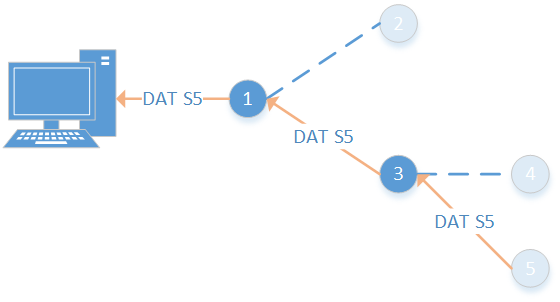
\includegraphics[scale=0.6]{content/images/Collection/Part6}
        \caption{Node 4 does not have any children so it sends its data and gets marked}
        \label{fig:coll6}
    \end{subfigure}
    \quad
    \quad
    \begin{subfigure}[t]{0.4\textwidth}
		\centering         
        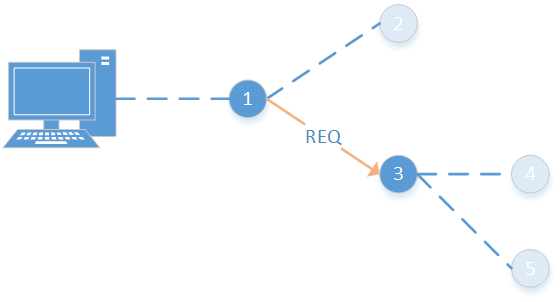
\includegraphics[scale=0.6]{content/images/Collection/Part7}
        \caption{Node 3 is still not marked so node 1 sends a request to it}
        \label{fig:coll7}
    \end{subfigure}
    \quad
    \quad
    \begin{subfigure}[t]{0.4\textwidth}
		\centering         
        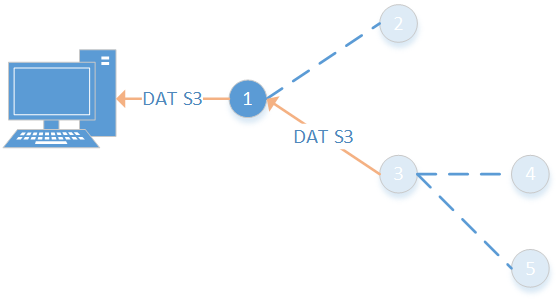
\includegraphics[scale=0.6]{content/images/Collection/Part8}
        \caption{All the children of node 3 are marked so it starts sending its data and gets marked itself}
        \label{fig:coll8}
    \end{subfigure}
    \quad
    \quad
    \begin{subfigure}[t]{0.4\textwidth}
		\centering         
        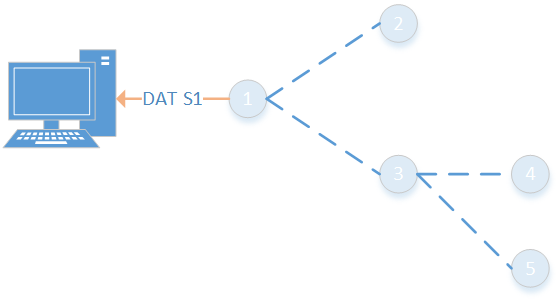
\includegraphics[scale=0.6]{content/images/Collection/Part9}
        \caption{Now all the children of node 1 are marked and it can send its own data to the base station and gets marked}
        \label{fig:coll9}
    \end{subfigure}
    \caption{This is an example for the collection. REQ means request and DAT Sx stands for data from source x}
\end{figure}

To collect the data from the network, we make use of the created paths and their tree structure. The process is shown in Figure \ref{fig:coll}. The Figure shows a wireless sensor network represented by the nodes and the paths to the sink created in the calibration phase. Note that the nodes could also have other connections between each other. 

To start the collection the sink sends a request to one of its children. The child receiving that request will check if it has any children himself and if that is the case, it will forward the request to one of them. When the request reaches a node without any children, the node will send its data to its parent which forwards the data to its parent, until the data reaches the sink, which will forward it to the base station. Every node that receives a data message marks the source of that data as done. When the sink sent the received data to the base station, it  sends a new request to one of its children that has not been marked as done. That child again forwards that request to a child that has not been marked as done. If the request reaches a node that has no children or every child has been marked as done it sends its own data. This process will be repeated until the sink does not have any more children left that are not marked as done. Then the sink can send its own data to the base station and finish the collection. All nodes now need to unmark all the other nodes, so another collection is possible.

\section{Creating the Schedule}
\label{chp:apr_creatingSchedule}
Creating a schedule is a quite challenging task since we need an algorithm that visits every node in a graph at least once and starts and ends at the same node. The optimal schedule would be a Hamilton-Circle that is a circle inside a graph that visits each node exactly once. To figure out if a Hamilton-Circle exists, there is however only the way to bruteforce all the possible combinations. This is highly inefficient and possibly we do not even get a result at the end. Therefore this thesis suggests a simple method that makes sure every node gets visited at least once and the path starts and ends at the same node. This method however is not able to create an optimal path and could be improved.

\subsection{Rooted Circles}
\begin{figure}[htbp]
	\centering
	\begin{subfigure}[t]{0.4\textwidth}
		\centering
    		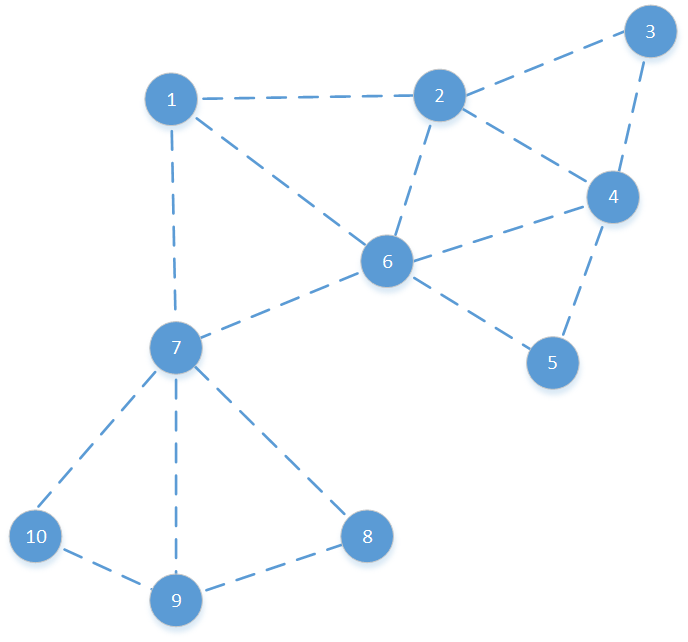
\includegraphics[scale=0.6]{content/images/Schedule/Network}
   	 	\caption{The example network with all its connections between nodes}
    	\label{fig:network}
    \end{subfigure}
    \quad
    \quad
    \begin{subfigure}[t]{0.4\textwidth}
		\centering         
        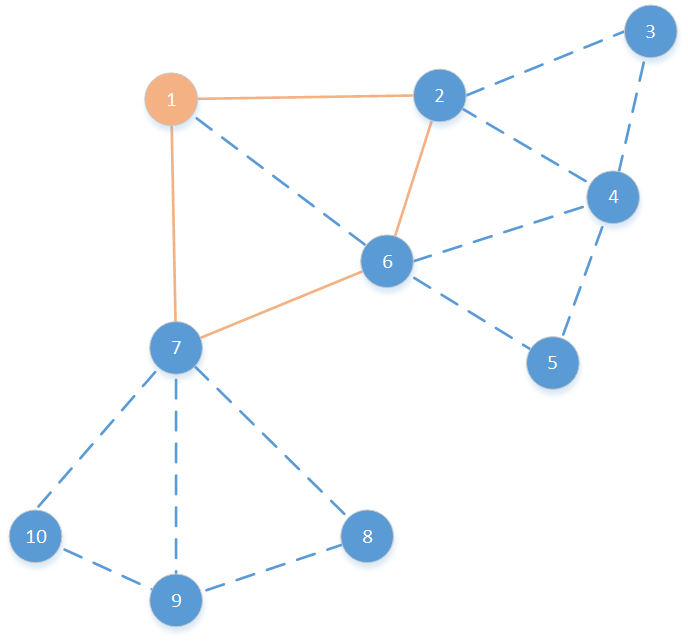
\includegraphics[scale=0.6]{content/images/Schedule/RootedCircle}
        \caption{Example for a rooted circle with node 1 as the root}
        \label{fig:rootedCircle}
    \end{subfigure}
    \label{fig:networkRootedCircle}
    \caption{A rooted circle inside a example network}
\end{figure}

The suggested method is based on smaller circles inside the graph. These circles will have a root node that is the start and the end point of the circle. All the nodes inside this circle will be in range of the root of the circle. These circles will be called rooted circles. In Figure \ref{fig:rootedCircle} such a rooted circle is represented inside the network depicted in Figure \ref{fig:network}. To create a rooted circle, one node needs to be chosen as the root. Then the root will take one node from its neighbour table and choose it as the second node in the circle.  Then the second node will look into its neighbour table and choose a node that has the root node inside its neighbour table. The chosen node will do the same and the process will be repeated until a node does not have a neighbour that has the root as a neighbour. Then the circle will be closed and the path goes to the root. When we look at the example in Figure \ref{fig:rootedCircle} this means node 1 was chosen as the root. Then node 2 was picked as the second node in the circle. Node 2 has multiple neighbours but only one of them, node 6, has the root node 1 as a neighbour. This means node 6 is chosen as the next node in the circle. Node 6 now has node 2 and node 7 as neighbours that also have the root as a neighbour, however node 2 is already inside the circle so node 7 is chosen as the next node. Node 7 now has no more neighbours that have the root as a neighbour and the circle is closed.

\subsection{Creating a Full Schedule}
\begin{figure}[htbp]
	\centering         
    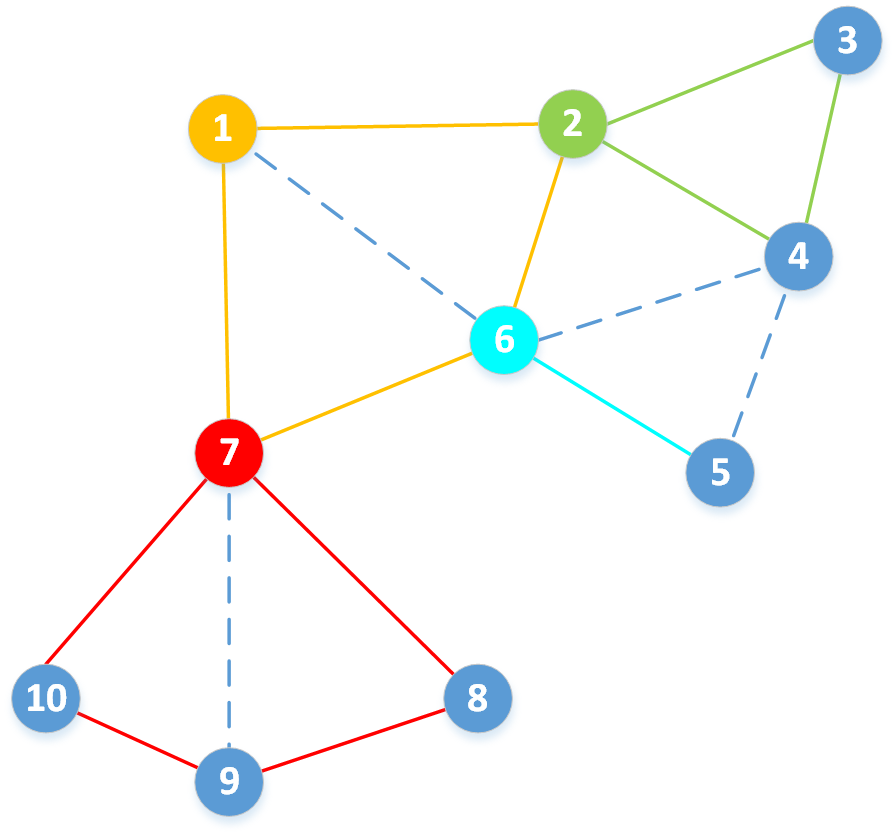
\includegraphics[scale=0.6]{content/images/Schedule/FullSchedule}
    \caption{Full schedule for the example network of Figure \ref{fig:network}. The order in which the nodes send their messages would be: 1 2 3 4 2 6 5 6 7 8 9 10 7 1.}
    \label{fig:schedule}
\end{figure} 
We now want to fill the whole graph with rooted circles. Therefore we will choose the sink as the first root and create a rooted circle around it. When the circle is done, we will go through all the nodes of the circle and, if possible, create rooted circles around them as well. Then we do the same for all the new circles until every node was suggested as a root once. When creating new circles it is not possible to choose a node already inside another circle to be part of the new circle. In Figure \ref{fig:schedule} the network from Figure \ref{fig:network} is fully covered by rooted circles. The first circle created was the one that has node 1 as a root. Then all the nodes inside that circle where chosen as new roots to create new rooted circles. The first thing one could notice is that the circle with the root 6 only has one other node and does not really form a circle. This happens if the circle is closed directly after the second node following the root is chosen because there are no more neighbours left that also have the root as a neighbour. When running the schedule, this means a message would be sent from node 6 to node 5 and then from node 5 back to node 6. Also note that in theory there is a bigger rooted circle possible with the root 6 when node 4 would be included, but node 2 created its rooted circle first and included node 4 and therefore blocked it for rooted circles created at a later point in time. Listing 3.1 provides the pseudocode of an algorithm to cover a whole graph with rooted circles.

\lstset{caption={Pseudocode that covers a graph with rooted circles},label={lis:rooted}}
\begin{lstlisting}
RootedCircle createRootedCircle(Node root) {
	Node node = getNextForCircle(root, root)	

	If(node != null) {
		RootedCircle rootedCircle = new rootedCircle(root)
		rootedCircle.addNode(node)
		node.setPartOfCircle(true)

		while((node = getNextForCircle(root, node, rootedCircle)) != null) {
			rootedCircle.add(node)
			node.setPartOfCircle(true)
		}

		return rootedCircle
	} else {
		return null
	}
}

Node getNextForCircle(Node root, Node neighbour) {
	for each (Node node in root.getNeighbourList)	
		if(node.isNeighbourOf(neighbour) and not node.isPartOfACircle())
			return node
	return null
}

List<RootedCircle> coverGraphWithRootedCircles(Node firstRoot) {
	List<RootedCircle> circleList = new List<RootedCircle()>
	
	circleList.add(createRootedCircle(firstRoot))

	for each (RootedCircle circle in circleList) {
		for each (Node node in circle) {
			RootedCircle newCircle = createRootedCircle(node)
			if(newCircle != null)
				circleList.add(newCircle);
		}
	}
}
\end{lstlisting}

\section{Spreading the Schedule}
\label{chp:apr_spreadingSchedule}
To spread the schedule we will again make use of the tree structure of the created path. When the sink received the schedule from the base station it will forward it to its first child. The child will forward it to one of his children and so on. When a node that received the schedule has no more children, it will send the schedule back to its parent. The parent receiving the schedule will now forward the schedule to its next child. If a parent received the schedule back from all its children, it will forward it to its own parent. In Figure \ref{fig:spreading} an example for this process is given. The Figure shows a wireless sensor network represented by the nodes and the paths to the sink created in the calibration phase. Note that the nodes could also have other connections between each other. 

When you look at the example, one can see that already in Figure \ref{fig:spreading7} the schedule is received by all the nodes but still there are messages sent that could seem useless at this point. However at this point in time we do not know if the sink has any more children that did not receive the schedule yet. Therefore the schedule needs to travel all the way back to the sink. Only at the moment the schedule reaches the sink and the sink does not have any more children left that need to receive the schedule, we know for sure that the schedule is fully spread.

\begin{figure}[htbp]
	\centering
	\begin{subfigure}[t]{0.4\textwidth}
		\centering
    		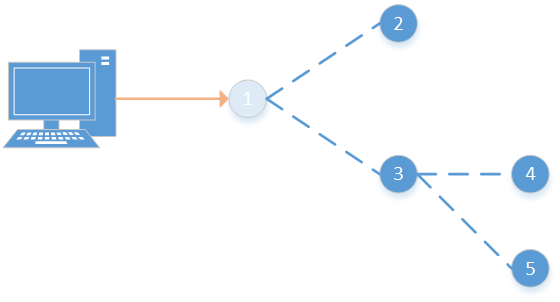
\includegraphics[scale=0.6]{content/images/ScheduleSpreading/Part1}
   	 	\caption{The base station sends the schedule to node 1.}
    	\label{fig:spreading1}
    \end{subfigure}
    \quad
    \quad
    \begin{subfigure}[t]{0.4\textwidth}
		\centering         
        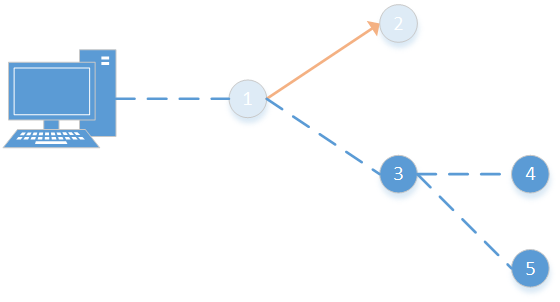
\includegraphics[scale=0.6]{content/images/ScheduleSpreading/Part2}
        \caption{Node 1 forwards the schedule to node 2}
        \label{fig:spreading2}
    \end{subfigure}
    \quad
    \quad
    \begin{subfigure}[t]{0.4\textwidth}
		\centering         
        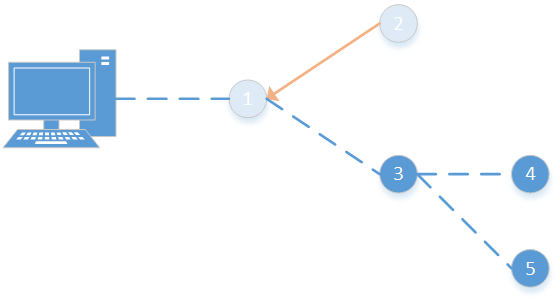
\includegraphics[scale=0.6]{content/images/ScheduleSpreading/Part3}
        \caption{Node 2 does not have any children and sends the schedule to its parent node 1}
        \label{fig:spreading3}
    \end{subfigure}
    \quad
    \quad
    \begin{subfigure}[t]{0.4\textwidth}
		\centering         
        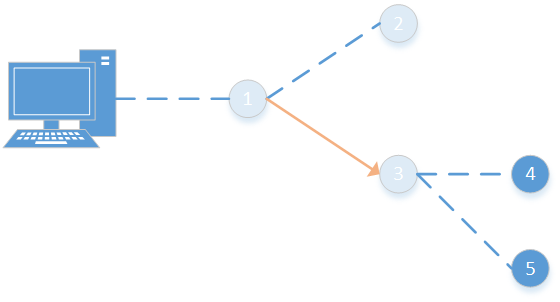
\includegraphics[scale=0.6]{content/images/ScheduleSpreading/Part4}
        \caption{Node 2 is now marked so node 1 will forward the schedule to node 3}
        \label{fig:spreading4}
    \end{subfigure}
    \quad
    \quad
    \begin{subfigure}[t]{0.4\textwidth}
		\centering         
        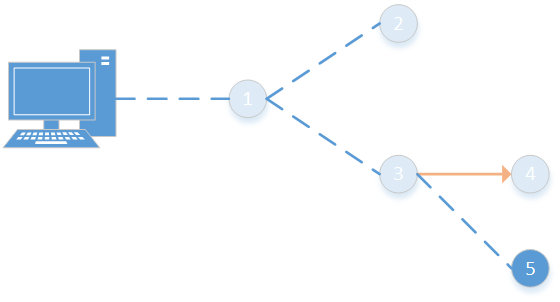
\includegraphics[scale=0.6]{content/images/ScheduleSpreading/Part5}
        \caption{Node 3 forwards the schedule to node 4}
        \label{fig:spreading5}
    \end{subfigure}
    \quad
    \quad
    \begin{subfigure}[t]{0.4\textwidth}
		\centering         
        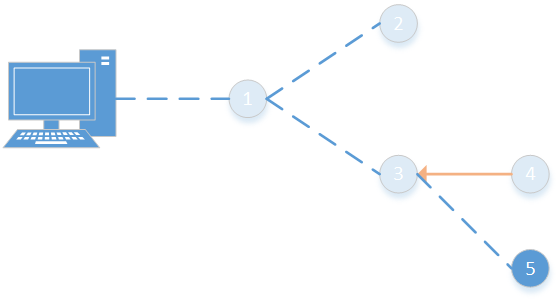
\includegraphics[scale=0.6]{content/images/ScheduleSpreading/Part6}
        \caption{Node 4 does not have any children and sends the schedule to its parent node 3}
        \label{fig:spreading6}
    \end{subfigure}
    \quad
    \quad
    \begin{subfigure}[t]{0.4\textwidth}
		\centering         
        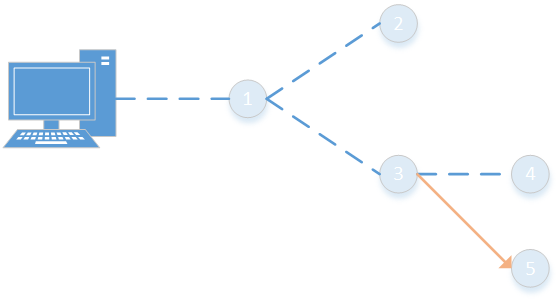
\includegraphics[scale=0.6]{content/images/ScheduleSpreading/Part7}
        \caption{Node 3 has still node 5 as an unmarked child and forwards the schedule to it}
        \label{fig:spreading7}
    \end{subfigure}
    \quad
    \quad
    \begin{subfigure}[t]{0.4\textwidth}
		\centering         
        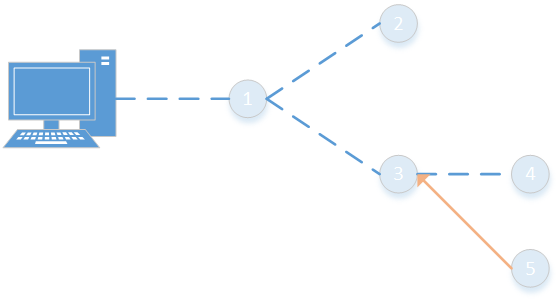
\includegraphics[scale=0.6]{content/images/ScheduleSpreading/Part8}
        \caption{Node 5 does not have any children and sends the schedule to its parent node 3}
        \label{fig:spreading8}
    \end{subfigure}
    \quad
    \quad
    \begin{subfigure}[t]{0.4\textwidth}
		\centering
    		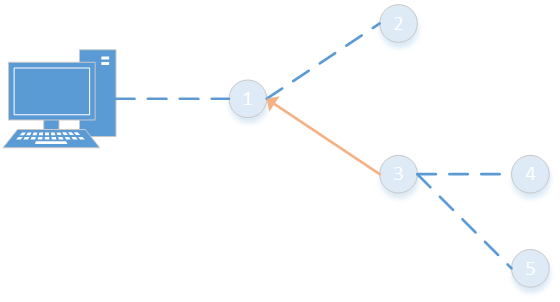
\includegraphics[scale=0.6]{content/images/ScheduleSpreading/Part9}
   	 	\caption{Node 3 has no more unmarked children and sends the schedule to its parent node 1}
    	\label{fig:spreading9}
    \end{subfigure}
    \quad
    \quad	
    \begin{subfigure}[t]{0.4\textwidth}
		\centering         
        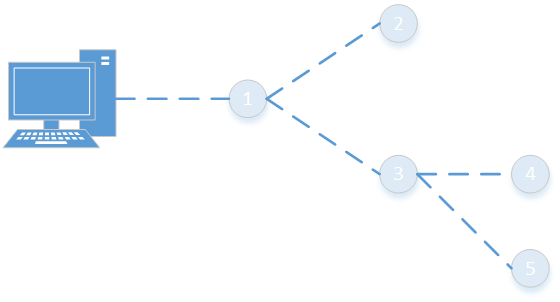
\includegraphics[scale=0.6]{content/images/ScheduleSpreading/Part10}
        \caption{Since node 1 does not have any more unmarked children the schedule is now fully spread inside the network}
        \label{fig:spreading10}
    \end{subfigure}
    \caption{This is an example for a path a schedule message takes to be spread inside the network}
     \label{fig:spreading}
\end{figure}

\section{Sampling}
When the schedule is spread and the sample module knows about the schedule and the neighbour list, the sampling can start. To do so the sink will send a  message like the on shown in Listing \ref{lis:sampleMsg} in Broadcast. The $receiver$ field will be set to the node id of the successor of the sink. Then all the nodes receiving the message will measure the received signal strength and save it inside their neighbour lists. After that each node that received the message will check if it is the successor by comparing its ID with the $receiver$ field inside the message. If a node recognizes itself as the successor of the sending node the node will evaluate the fitting successor, save it inside a new message and then also send it in broadcast. When the sink receives a message and does not have another successor it will signal the $finishedRound$ event.

\lstset{caption={Sample message structure},label={lis:sampleMsg}}
\begin{lstlisting}
	typedef nx_struct SampleMsg {
		nx_uint8_t receiver;
	}
\end{lstlisting} 

To evaluate the fitting successor the first approach coming to mind would be to just go through the schedule array and searching for the sending node followed by the searching nodes id. The successor then would be the node after that. This however is inefficient and unnecessarily stretches the timeslot to catch message drops. Therefore it is suggested to evaluate all the predecessors and successors of a node before the sampling starts by going through the whole schedule once and save them in a structure like the one shown in Listing \ref{lis:scheduleSaving} in the order of appearance. Additionally each node will store the index of the next predecessor successor pair that should appear. Then when a node is the successor it can simply check if the predecessor at the saved index is correct and if that is the case include the corresponding saved successor inside its message. After that the node can calculate the next index as
\[ I+1 = (I + 1)\%\mbox{numberOfPS}\]  
where $I$ is the current index and $numberOfPS$ the amount of predecessor successor pairs the node has stored. It can appear that the predecessor at the saved index is not corresponding to the sending node. This happens when a message drops and the node gets skipped.
In that case we have to go to all the predecessor successor pairs to find the right successor and adjust the saved index accordingly. However this is still much more efficient than going through the whole schedule.

\lstset{caption={Structures to save the successor and predecessors},label={lis:scheduleSaving}}
\begin{lstlisting}
	typedef struct PredecessorSuccessor {
		uint8_t predecessor;
		uint8_t successor;
	}

	typedef struct SchedulePSCollection {
		uint8_t numberOfPS;
		PredecessorSuccessor preSuc[MAX_PREDECESSORS_SUCCESSORS]; 
	}
\end{lstlisting}

To catch the message drops like explained in Chapter \ref{chp:apr_samplingDrops} whenever a node receives a message and is not the successor it needs to run through the schedule array and and calculate how many nodes send between the sending node and itself. Then the node has to calculate the time it takes for the schedule to reach the node. After that the node will start a timer that fires after exactly that time. Moreover the node needs to save the successor in case of the drop. The timer will be reset to the new time whenever the node receives a message. When the timer fires the node will simply send a message with the $receiver$ set as the saved successor.

 Since a node can appear multiple times inside the schedule it also needs to calculate the time to its next send directly after it send a message. If it does appear again in the schedule it will start the timer.  
